% Figure floats for the NeurReps Extended Abstract.
%
% % Figure floats for the NeurReps Extended Abstract.
%
% % Figure floats for the NeurReps Extended Abstract.
%
% % Figure floats for the NeurReps Extended Abstract.
%
% \input{figures} from the jmlr skeleton's body. Every float uses \floatconts, which the jmlr
% class provides, so captions sit above the graphic and \label lives inside the float.
%
% The \includegraphics filenames are the manifest names verbatim, hashes and arm counts included.
% They are ugly on purpose: the hash is the result set the figure was drawn from and the arm count
% is the n behind it, so a stale PDF cannot be swapped in without the filename changing. Do not
% rename them, and do not strip the hash to tidy the directory listing --- the correspondence to
% figures/MANIFEST.json is what makes the figure checkable, and scripts/check_submission.py
% verifies that every \includegraphics here names a file the manifest currently claims.
%
% Captions are the drafts in docs/07-writeup.md sections D and E, with citations attached.

\begin{figure}[t]
\floatconts
  {fig:decomposition}
  {\caption{\textbf{Forgetting decomposes exactly, and the channel that carries it shifts with
   richness.} Retained capacity for task~0 at lag~12, decomposed by the exact identity of
   \citet{chou2026diagnosing}. Pooled over the three conditions that lose capacity (24 unique seeds
   per $\gamma_0$; 120 files are five copies); \texttt{S-HH} is Figure~\ref{fig:benign}.
   \textbf{(a)}~Magnitude in noise floors, signed: 0.2 at $\gamma_0=0.03$ to 69.7 at $\gamma_0=10$.
   Grey band: $\pm 2$ floors.
   \textbf{(b)}~Channel shares, $|\mathrm{term}|/\sum|\mathrm{term}|$, drawn where the total clears
   the band. $\gamma_0=0.1$ hatched (margin inside the floor's uncertainty); $\gamma_0=0.3$ and
   above solid: utility $0.08\to0.45$, radius $0.39\to0.11$, dimension $0.53\to0.44$ then flat.
   \textbf{(c)}~Signed terms; utility negative on 100\% of arms for $\gamma_0\geq 1$.
   \textbf{(d)}~Center-collapse share of the radius channel, $0.05\to0.44$ through $\gamma_0=3$ then
   flat ($\gamma_0=3\to10$ step unresolved, CI $[-0.038,+0.070]$). Each bar gated at $3\times$ its
   own $R_{\mathrm{eff}}$ floor; coverage is not comparable across bars.
   Lag~12 exists only for task~0, the most-forgotten task --- the largest forgetting in the grid,
   not its average.}}
  {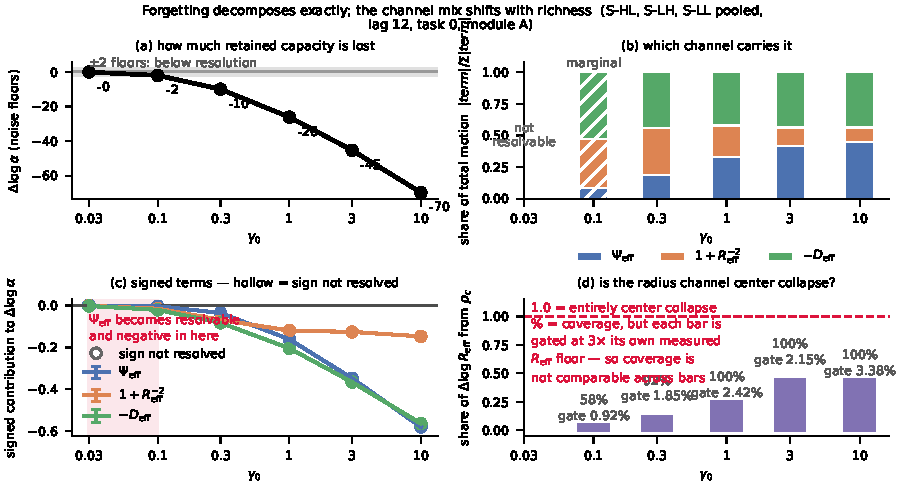
\includegraphics[width=\linewidth]
   {figures/fig2_gamma_sweep__forgetting__lag12__960arms__8dd793134c38.pdf}}
\end{figure}

\begin{figure}[t]
\floatconts
  {fig:corners}
  {\caption{\textbf{Center correlation moves in opposite directions across the similarity design,
   and the two axes act almost separately.}
   \textbf{(a)}~Signed $\rho_c$ at $\gamma_0=10$, design of \citet{hiratani2024disentangling}. All
   four corners start together ($\rho_c = 0.391$--$0.392$); three converge, \texttt{S-HL} (same
   stimuli, different rules) decorrelates.
   \textbf{(b)}~Grey band: lazy-arm drift ($\gamma_0=0.03$). \texttt{S-LL} never leaves it.
   \textbf{(c)}~\texttt{S-HL} decline is progressive, negative on 8 of 8 unique seeds
   ($p=0.0078$, the floor of a two-sided sign test at $n=8$; 40 files are copies), median Spearman
   $-0.79$.
   \textbf{(d)}~H1d and H6 fail in sign: three of four corners converge; largest $|\Delta\rho_c|$ is
   \texttt{S-LH}, twice \texttt{S-HL}.
   \textbf{(e)}~Readout $+0.104$, feature $-0.061$, interaction $+0.006$; additive error $0.012$.
   \textbf{(f)}~Both main effects survive a $4\times$ width change, ordering unchanged.}}
  {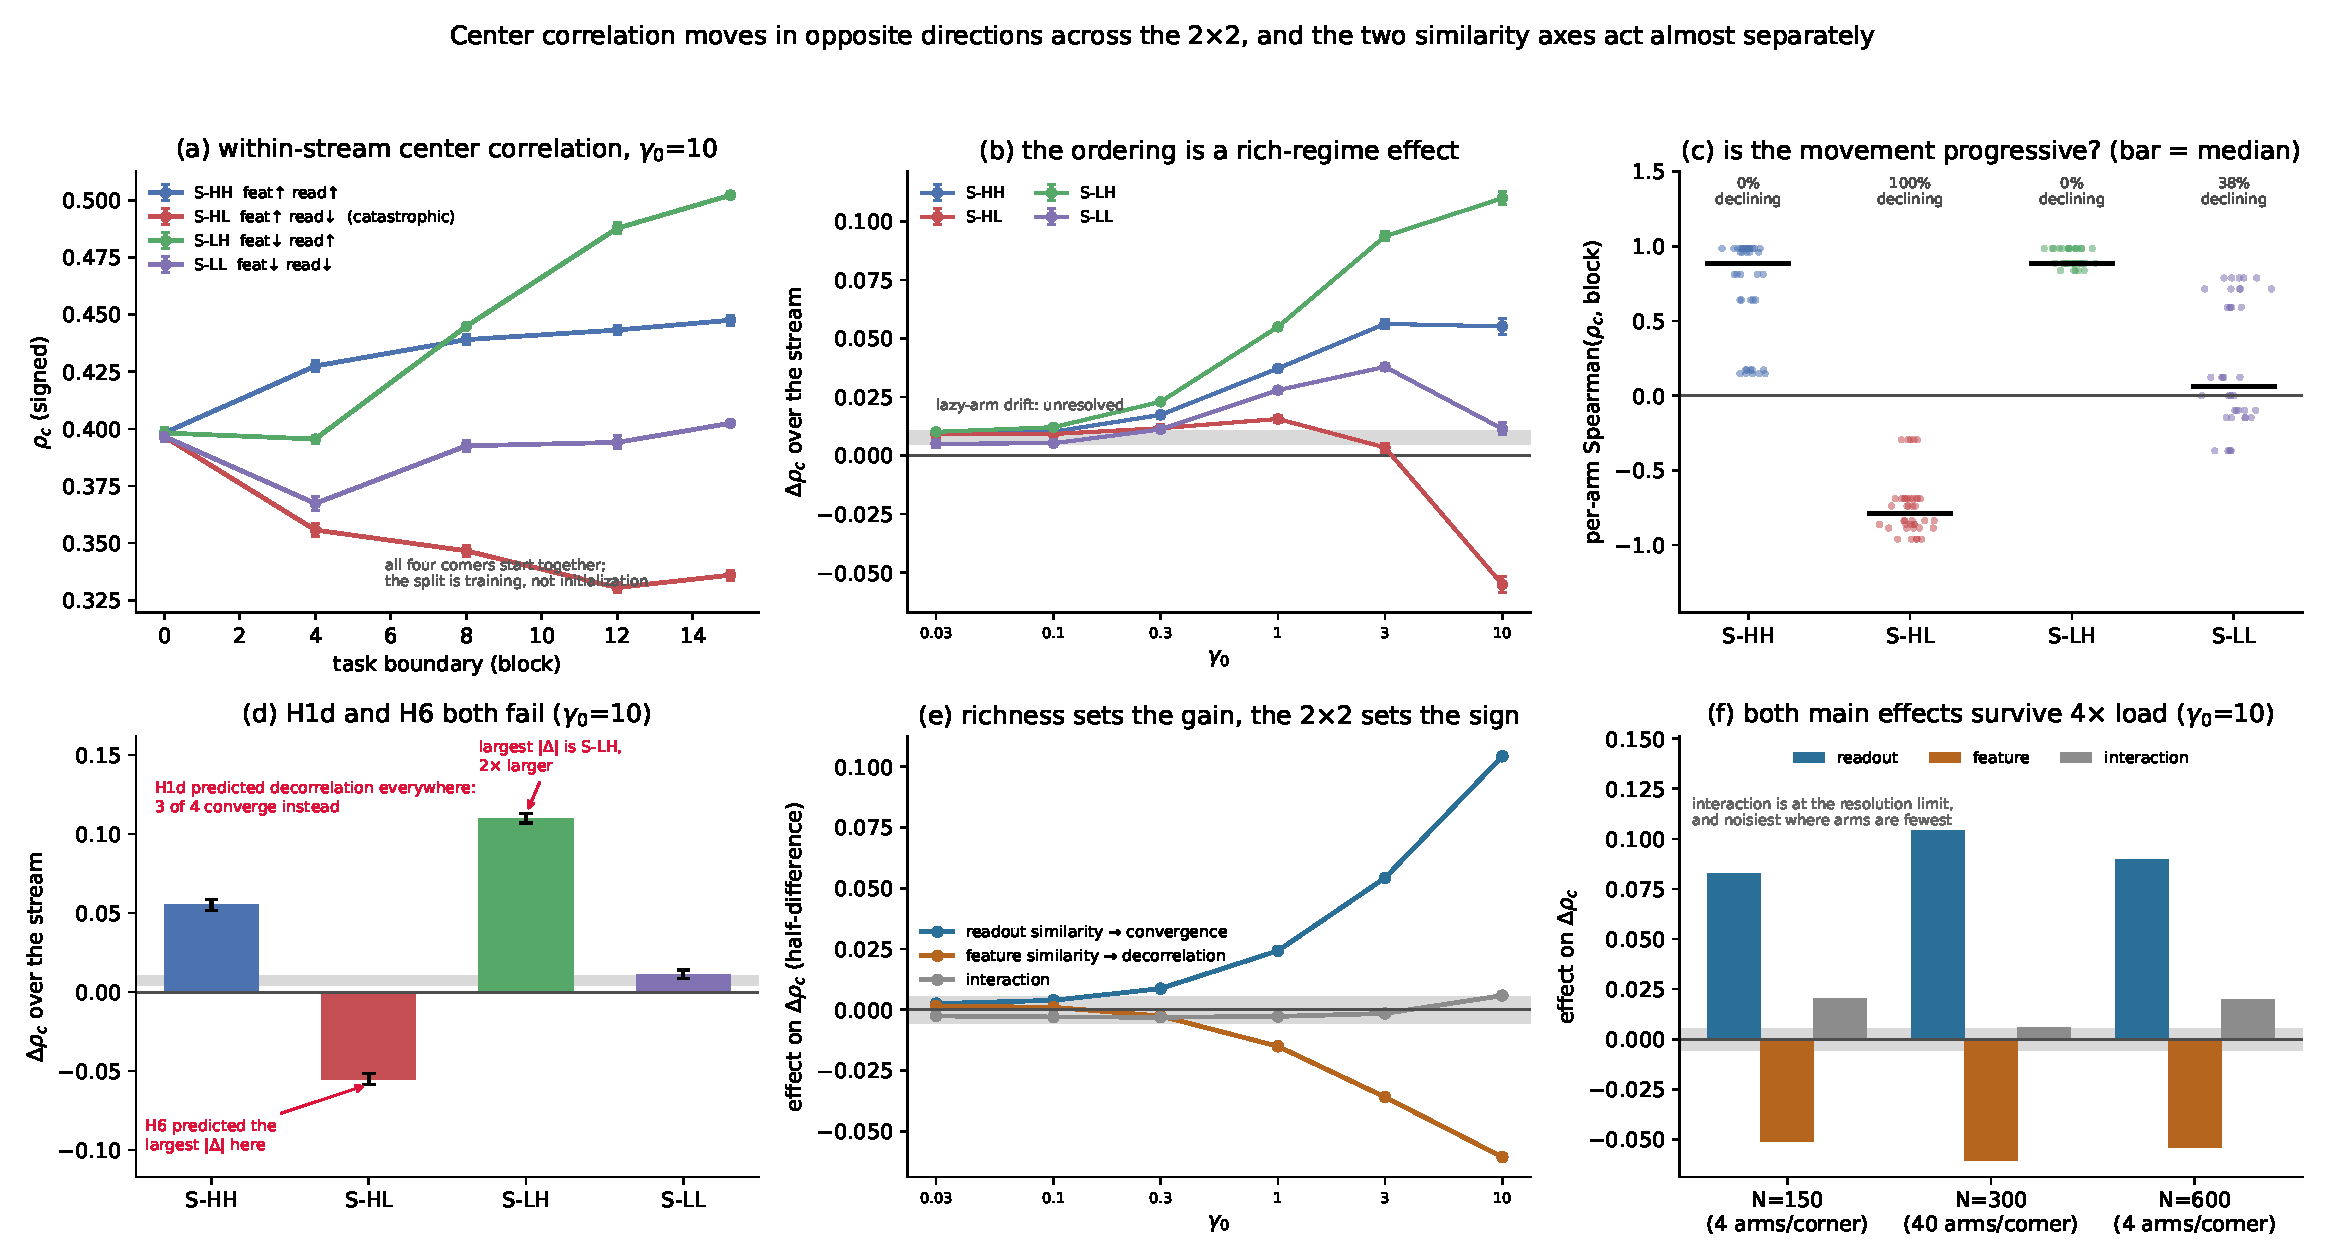
\includegraphics[width=\linewidth]
   {figures/fig4_corners_rho_c__gamma10__960arms__8dd793134c38.pdf}}
\end{figure}
 from the jmlr skeleton's body. Every float uses \floatconts, which the jmlr
% class provides, so captions sit above the graphic and \label lives inside the float.
%
% The \includegraphics filenames are the manifest names verbatim, hashes and arm counts included.
% They are ugly on purpose: the hash is the result set the figure was drawn from and the arm count
% is the n behind it, so a stale PDF cannot be swapped in without the filename changing. Do not
% rename them, and do not strip the hash to tidy the directory listing --- the correspondence to
% figures/MANIFEST.json is what makes the figure checkable, and scripts/check_submission.py
% verifies that every \includegraphics here names a file the manifest currently claims.
%
% Captions are the drafts in docs/07-writeup.md sections D and E, with citations attached.

\begin{figure}[t]
\floatconts
  {fig:decomposition}
  {\caption{\textbf{Forgetting decomposes exactly, and the channel that carries it shifts with
   richness.} Retained capacity for task~0 at lag~12, decomposed by the exact identity of
   \citet{chou2026diagnosing}. Pooled over the three conditions that lose capacity (24 unique seeds
   per $\gamma_0$; 120 files are five copies); \texttt{S-HH} is Figure~\ref{fig:benign}.
   \textbf{(a)}~Magnitude in noise floors, signed: 0.2 at $\gamma_0=0.03$ to 69.7 at $\gamma_0=10$.
   Grey band: $\pm 2$ floors.
   \textbf{(b)}~Channel shares, $|\mathrm{term}|/\sum|\mathrm{term}|$, drawn where the total clears
   the band. $\gamma_0=0.1$ hatched (margin inside the floor's uncertainty); $\gamma_0=0.3$ and
   above solid: utility $0.08\to0.45$, radius $0.39\to0.11$, dimension $0.53\to0.44$ then flat.
   \textbf{(c)}~Signed terms; utility negative on 100\% of arms for $\gamma_0\geq 1$.
   \textbf{(d)}~Center-collapse share of the radius channel, $0.05\to0.44$ through $\gamma_0=3$ then
   flat ($\gamma_0=3\to10$ step unresolved, CI $[-0.038,+0.070]$). Each bar gated at $3\times$ its
   own $R_{\mathrm{eff}}$ floor; coverage is not comparable across bars.
   Lag~12 exists only for task~0, the most-forgotten task --- the largest forgetting in the grid,
   not its average.}}
  {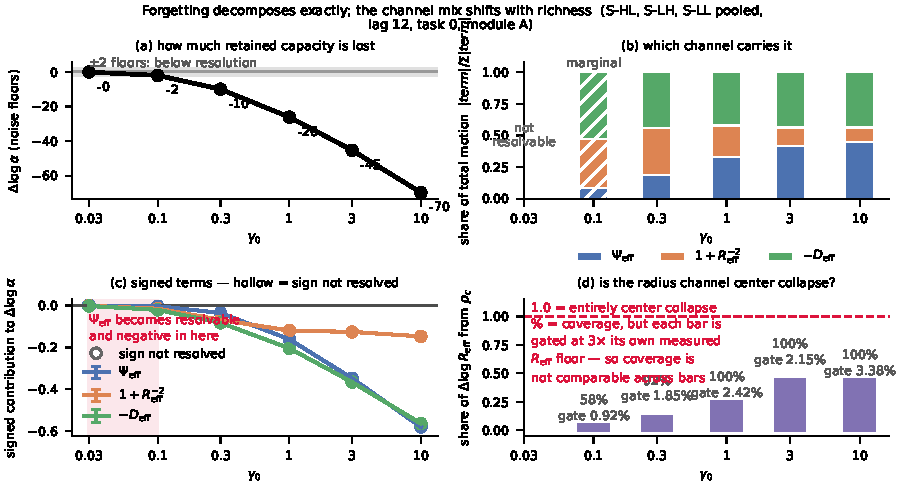
\includegraphics[width=\linewidth]
   {figures/fig2_gamma_sweep__forgetting__lag12__960arms__8dd793134c38.pdf}}
\end{figure}

\begin{figure}[t]
\floatconts
  {fig:corners}
  {\caption{\textbf{Center correlation moves in opposite directions across the similarity design,
   and the two axes act almost separately.}
   \textbf{(a)}~Signed $\rho_c$ at $\gamma_0=10$, design of \citet{hiratani2024disentangling}. All
   four corners start together ($\rho_c = 0.391$--$0.392$); three converge, \texttt{S-HL} (same
   stimuli, different rules) decorrelates.
   \textbf{(b)}~Grey band: lazy-arm drift ($\gamma_0=0.03$). \texttt{S-LL} never leaves it.
   \textbf{(c)}~\texttt{S-HL} decline is progressive, negative on 8 of 8 unique seeds
   ($p=0.0078$, the floor of a two-sided sign test at $n=8$; 40 files are copies), median Spearman
   $-0.79$.
   \textbf{(d)}~H1d and H6 fail in sign: three of four corners converge; largest $|\Delta\rho_c|$ is
   \texttt{S-LH}, twice \texttt{S-HL}.
   \textbf{(e)}~Readout $+0.104$, feature $-0.061$, interaction $+0.006$; additive error $0.012$.
   \textbf{(f)}~Both main effects survive a $4\times$ width change, ordering unchanged.}}
  {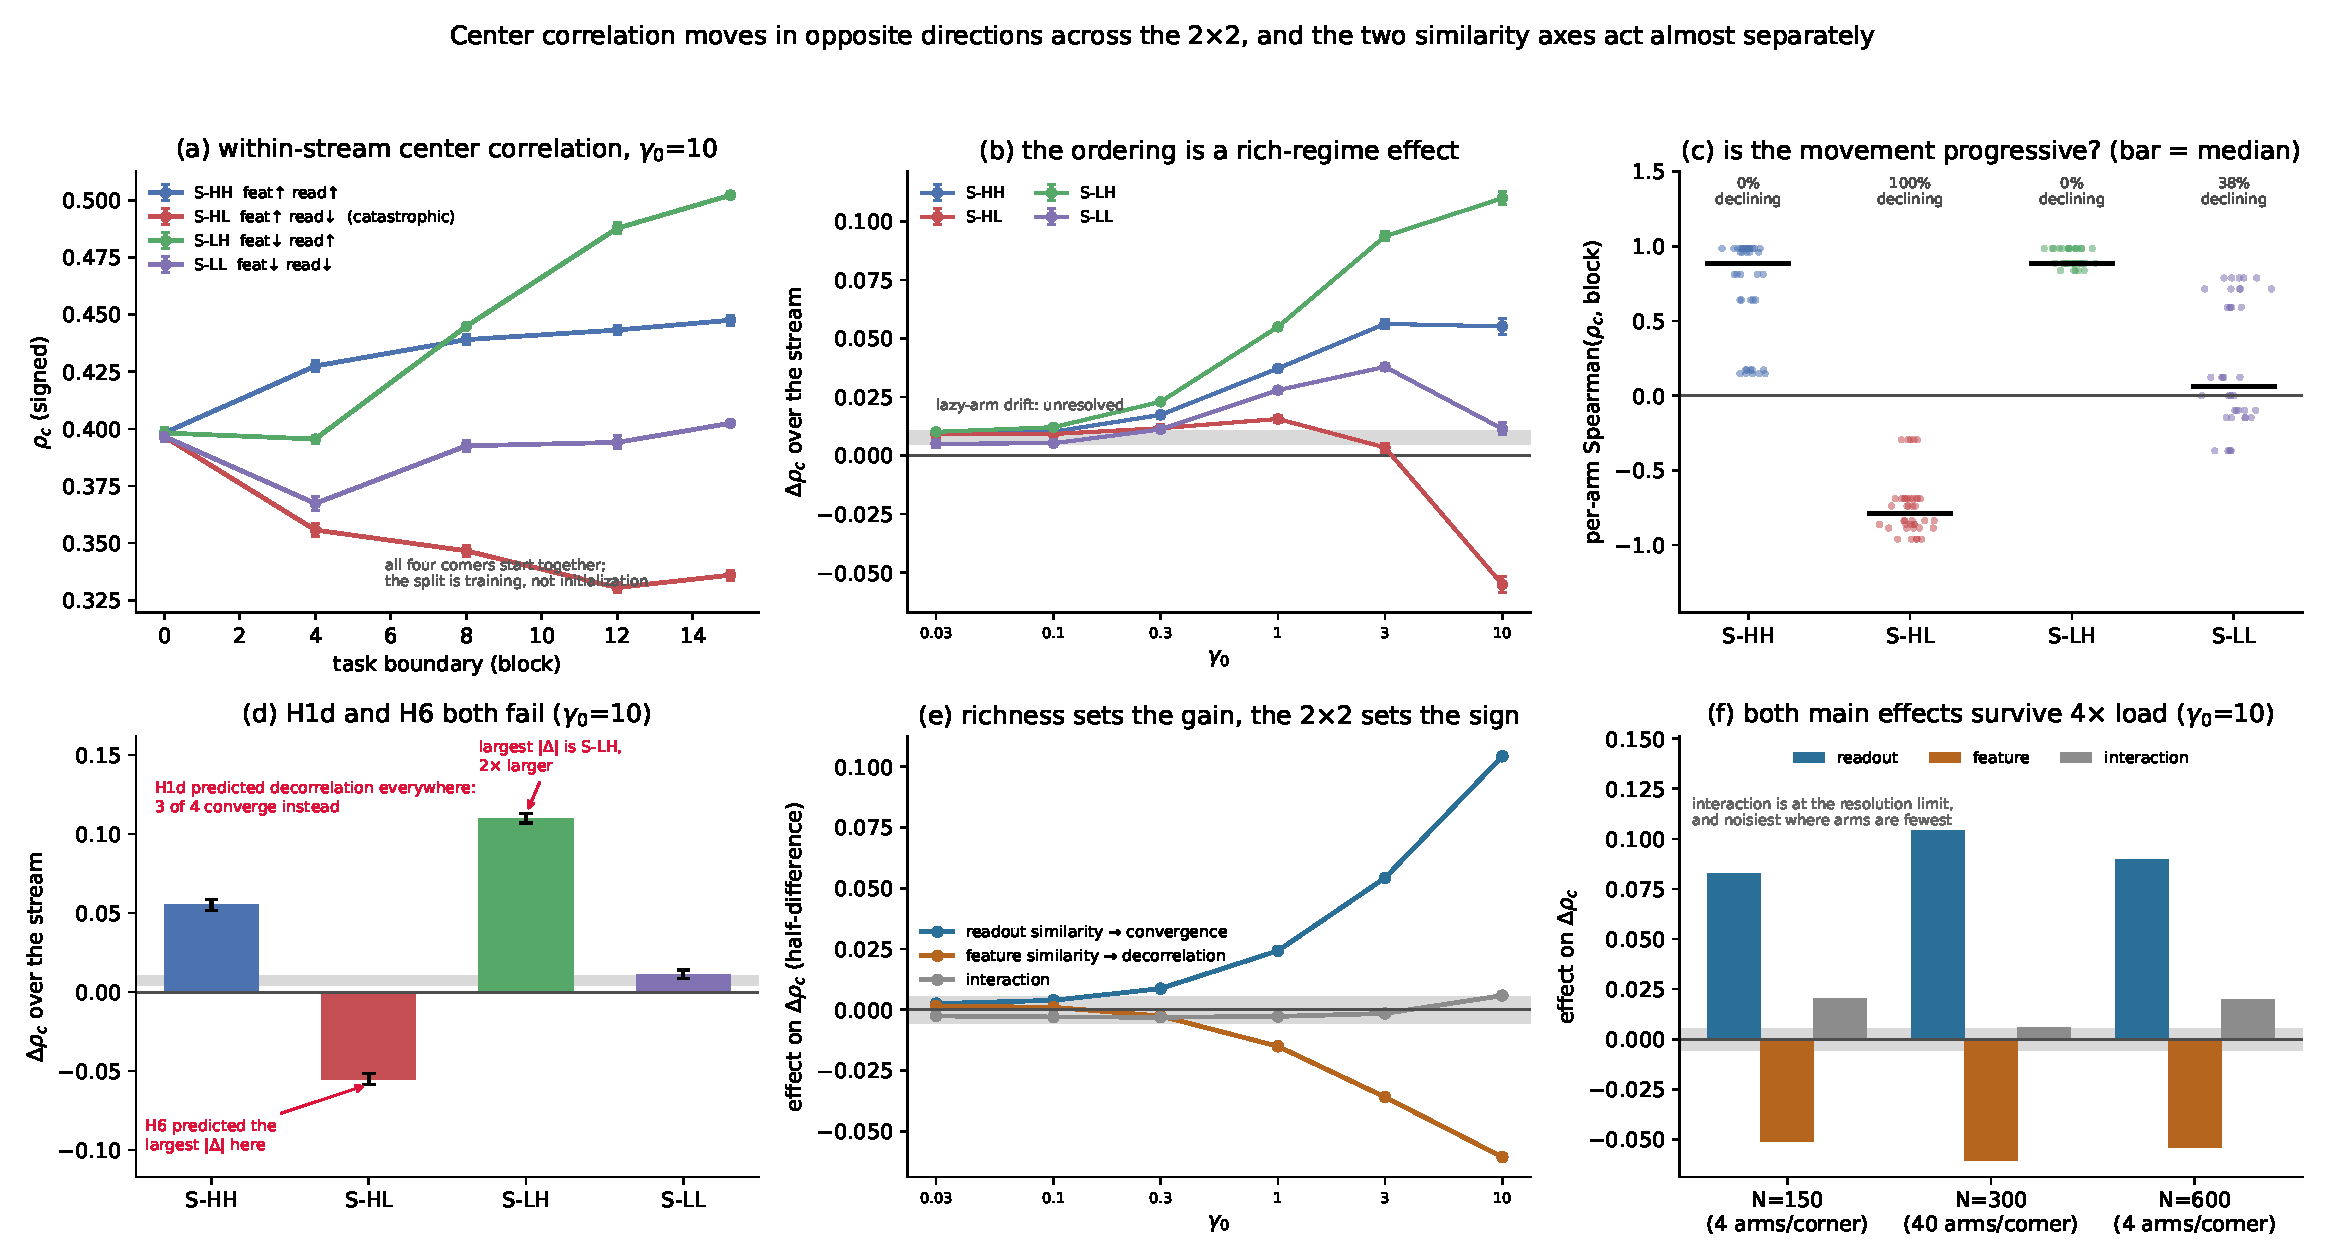
\includegraphics[width=\linewidth]
   {figures/fig4_corners_rho_c__gamma10__960arms__8dd793134c38.pdf}}
\end{figure}
 from the jmlr skeleton's body. Every float uses \floatconts, which the jmlr
% class provides, so captions sit above the graphic and \label lives inside the float.
%
% The \includegraphics filenames are the manifest names verbatim, hashes and arm counts included.
% They are ugly on purpose: the hash is the result set the figure was drawn from and the arm count
% is the n behind it, so a stale PDF cannot be swapped in without the filename changing. Do not
% rename them, and do not strip the hash to tidy the directory listing --- the correspondence to
% figures/MANIFEST.json is what makes the figure checkable, and scripts/check_submission.py
% verifies that every \includegraphics here names a file the manifest currently claims.
%
% Captions are the drafts in docs/07-writeup.md sections D and E, with citations attached.

\begin{figure}[t]
\floatconts
  {fig:decomposition}
  {\caption{\textbf{Forgetting decomposes exactly, and the channel that carries it shifts with
   richness.} Retained capacity for task~0 at lag~12, decomposed by the exact identity of
   \citet{chou2026diagnosing}. Pooled over the three conditions that lose capacity (24 unique seeds
   per $\gamma_0$; 120 files are five copies); \texttt{S-HH} is Figure~\ref{fig:benign}.
   \textbf{(a)}~Magnitude in noise floors, signed: 0.2 at $\gamma_0=0.03$ to 69.7 at $\gamma_0=10$.
   Grey band: $\pm 2$ floors.
   \textbf{(b)}~Channel shares, $|\mathrm{term}|/\sum|\mathrm{term}|$, drawn where the total clears
   the band. $\gamma_0=0.1$ hatched (margin inside the floor's uncertainty); $\gamma_0=0.3$ and
   above solid: utility $0.08\to0.45$, radius $0.39\to0.11$, dimension $0.53\to0.44$ then flat.
   \textbf{(c)}~Signed terms; utility negative on 100\% of arms for $\gamma_0\geq 1$.
   \textbf{(d)}~Center-collapse share of the radius channel, $0.05\to0.44$ through $\gamma_0=3$ then
   flat ($\gamma_0=3\to10$ step unresolved, CI $[-0.038,+0.070]$). Each bar gated at $3\times$ its
   own $R_{\mathrm{eff}}$ floor; coverage is not comparable across bars.
   Lag~12 exists only for task~0, the most-forgotten task --- the largest forgetting in the grid,
   not its average.}}
  {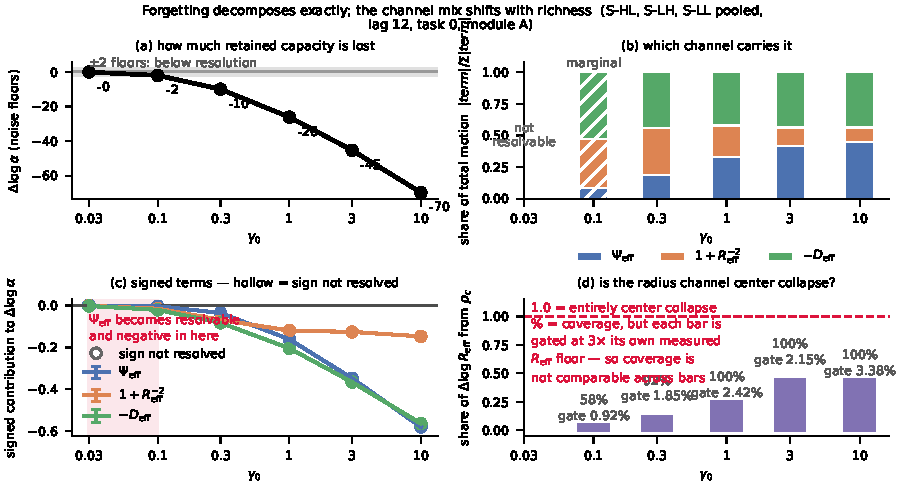
\includegraphics[width=\linewidth]
   {figures/fig2_gamma_sweep__forgetting__lag12__960arms__8dd793134c38.pdf}}
\end{figure}

\begin{figure}[t]
\floatconts
  {fig:corners}
  {\caption{\textbf{Center correlation moves in opposite directions across the similarity design,
   and the two axes act almost separately.}
   \textbf{(a)}~Signed $\rho_c$ at $\gamma_0=10$, design of \citet{hiratani2024disentangling}. All
   four corners start together ($\rho_c = 0.391$--$0.392$); three converge, \texttt{S-HL} (same
   stimuli, different rules) decorrelates.
   \textbf{(b)}~Grey band: lazy-arm drift ($\gamma_0=0.03$). \texttt{S-LL} never leaves it.
   \textbf{(c)}~\texttt{S-HL} decline is progressive, negative on 8 of 8 unique seeds
   ($p=0.0078$, the floor of a two-sided sign test at $n=8$; 40 files are copies), median Spearman
   $-0.79$.
   \textbf{(d)}~H1d and H6 fail in sign: three of four corners converge; largest $|\Delta\rho_c|$ is
   \texttt{S-LH}, twice \texttt{S-HL}.
   \textbf{(e)}~Readout $+0.104$, feature $-0.061$, interaction $+0.006$; additive error $0.012$.
   \textbf{(f)}~Both main effects survive a $4\times$ width change, ordering unchanged.}}
  {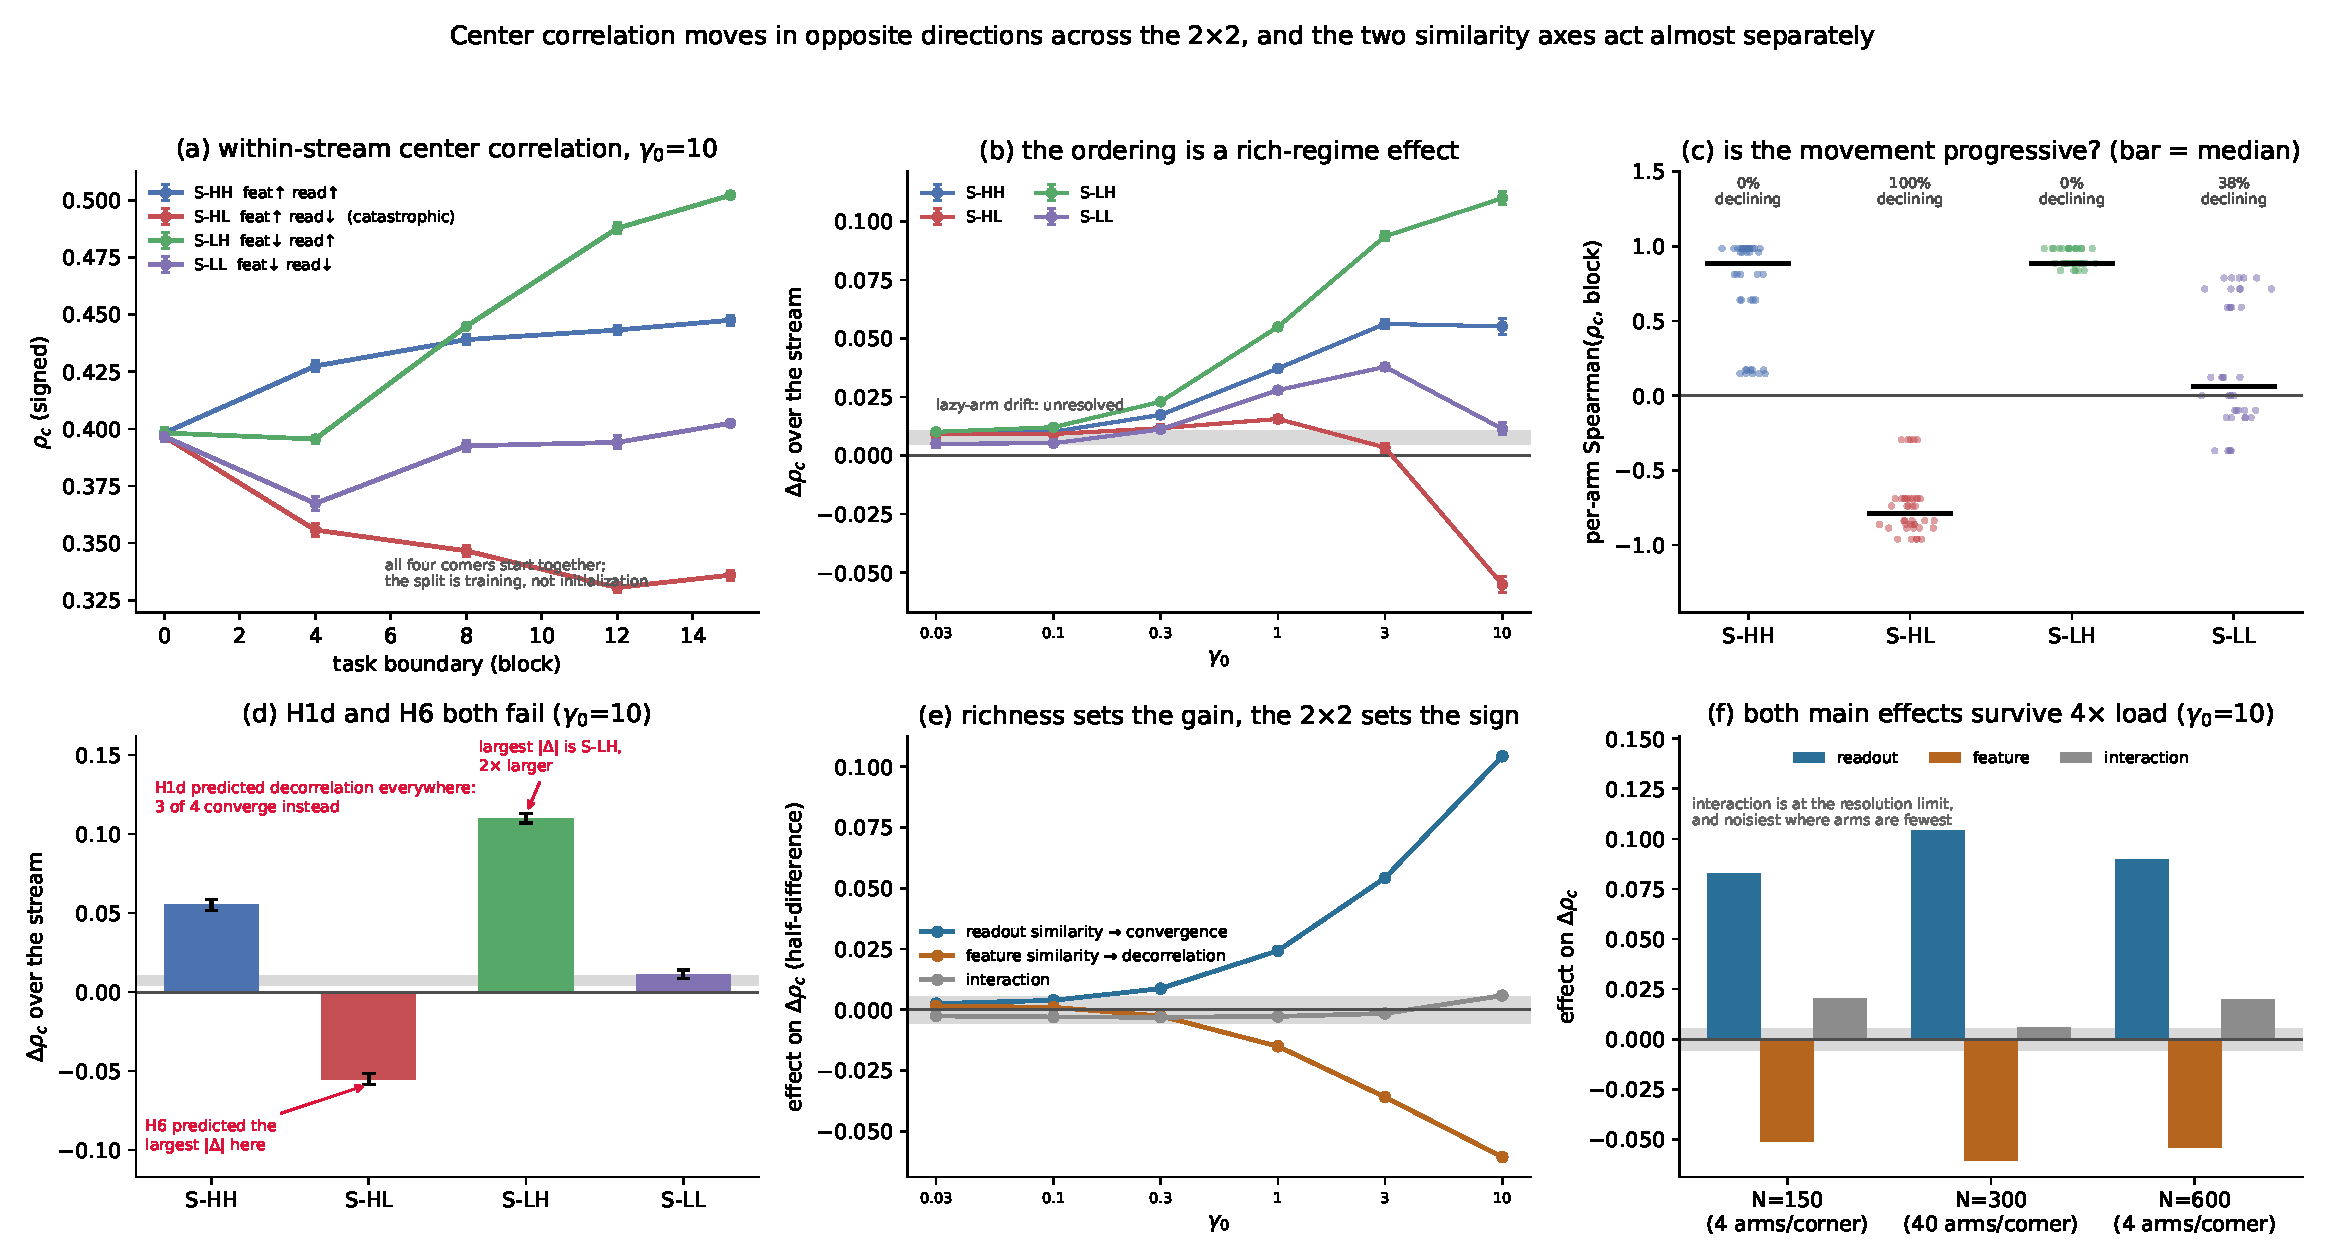
\includegraphics[width=\linewidth]
   {figures/fig4_corners_rho_c__gamma10__960arms__8dd793134c38.pdf}}
\end{figure}
 from the jmlr skeleton's body. Every float uses \floatconts, which the jmlr
% class provides, so captions sit above the graphic and \label lives inside the float.
%
% The \includegraphics filenames are the manifest names verbatim, hashes and arm counts included.
% They are ugly on purpose: the hash is the result set the figure was drawn from and the arm count
% is the n behind it, so a stale PDF cannot be swapped in without the filename changing. Do not
% rename them, and do not strip the hash to tidy the directory listing --- the correspondence to
% figures/MANIFEST.json is what makes the figure checkable, and scripts/check_submission.py
% verifies that every \includegraphics here names a file the manifest currently claims.
%
% Captions are the drafts in docs/07-writeup.md sections D and E, with citations attached.

\begin{figure}[t]
\floatconts
  {fig:decomposition}
  {\caption{\textbf{Forgetting decomposes exactly, and the channel that carries it shifts with
   richness.} Retained capacity for task~0 at lag~12, decomposed by the exact identity of
   \citet{chou2026diagnosing}. Pooled over the three conditions that lose capacity (24 unique seeds
   per $\gamma_0$; 120 files are five copies); \texttt{S-HH} is Figure~\ref{fig:benign}.
   \textbf{(a)}~Magnitude in noise floors, signed: 0.2 at $\gamma_0=0.03$ to 69.7 at $\gamma_0=10$.
   Grey band: $\pm 2$ floors.
   \textbf{(b)}~Channel shares, $|\mathrm{term}|/\sum|\mathrm{term}|$, drawn where the total clears
   the band. $\gamma_0=0.1$ hatched (margin inside the floor's uncertainty); $\gamma_0=0.3$ and
   above solid: utility $0.08\to0.45$, radius $0.39\to0.11$, dimension $0.53\to0.44$ then flat.
   \textbf{(c)}~Signed terms; utility negative on 100\% of arms for $\gamma_0\geq 1$.
   \textbf{(d)}~Center-collapse share of the radius channel, $0.05\to0.44$ through $\gamma_0=3$ then
   flat ($\gamma_0=3\to10$ step unresolved, CI $[-0.038,+0.070]$). Each bar gated at $3\times$ its
   own $R_{\mathrm{eff}}$ floor; coverage is not comparable across bars.
   Lag~12 exists only for task~0, the most-forgotten task --- the largest forgetting in the grid,
   not its average.}}
  {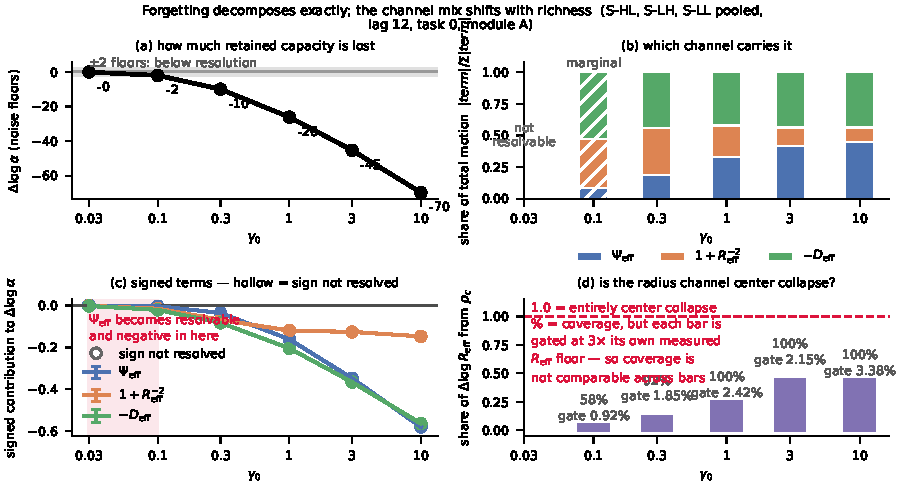
\includegraphics[width=\linewidth]
   {figures/fig2_gamma_sweep__forgetting__lag12__960arms__8dd793134c38.pdf}}
\end{figure}

\begin{figure}[t]
\floatconts
  {fig:corners}
  {\caption{\textbf{Center correlation moves in opposite directions across the similarity design,
   and the two axes act almost separately.}
   \textbf{(a)}~Signed $\rho_c$ at $\gamma_0=10$, design of \citet{hiratani2024disentangling}. All
   four corners start together ($\rho_c = 0.391$--$0.392$); three converge, \texttt{S-HL} (same
   stimuli, different rules) decorrelates.
   \textbf{(b)}~Grey band: lazy-arm drift ($\gamma_0=0.03$). \texttt{S-LL} never leaves it.
   \textbf{(c)}~\texttt{S-HL} decline is progressive, negative on 8 of 8 unique seeds
   ($p=0.0078$, the floor of a two-sided sign test at $n=8$; 40 files are copies), median Spearman
   $-0.79$.
   \textbf{(d)}~H1d and H6 fail in sign: three of four corners converge; largest $|\Delta\rho_c|$ is
   \texttt{S-LH}, twice \texttt{S-HL}.
   \textbf{(e)}~Readout $+0.104$, feature $-0.061$, interaction $+0.006$; additive error $0.012$.
   \textbf{(f)}~Both main effects survive a $4\times$ width change, ordering unchanged.}}
  {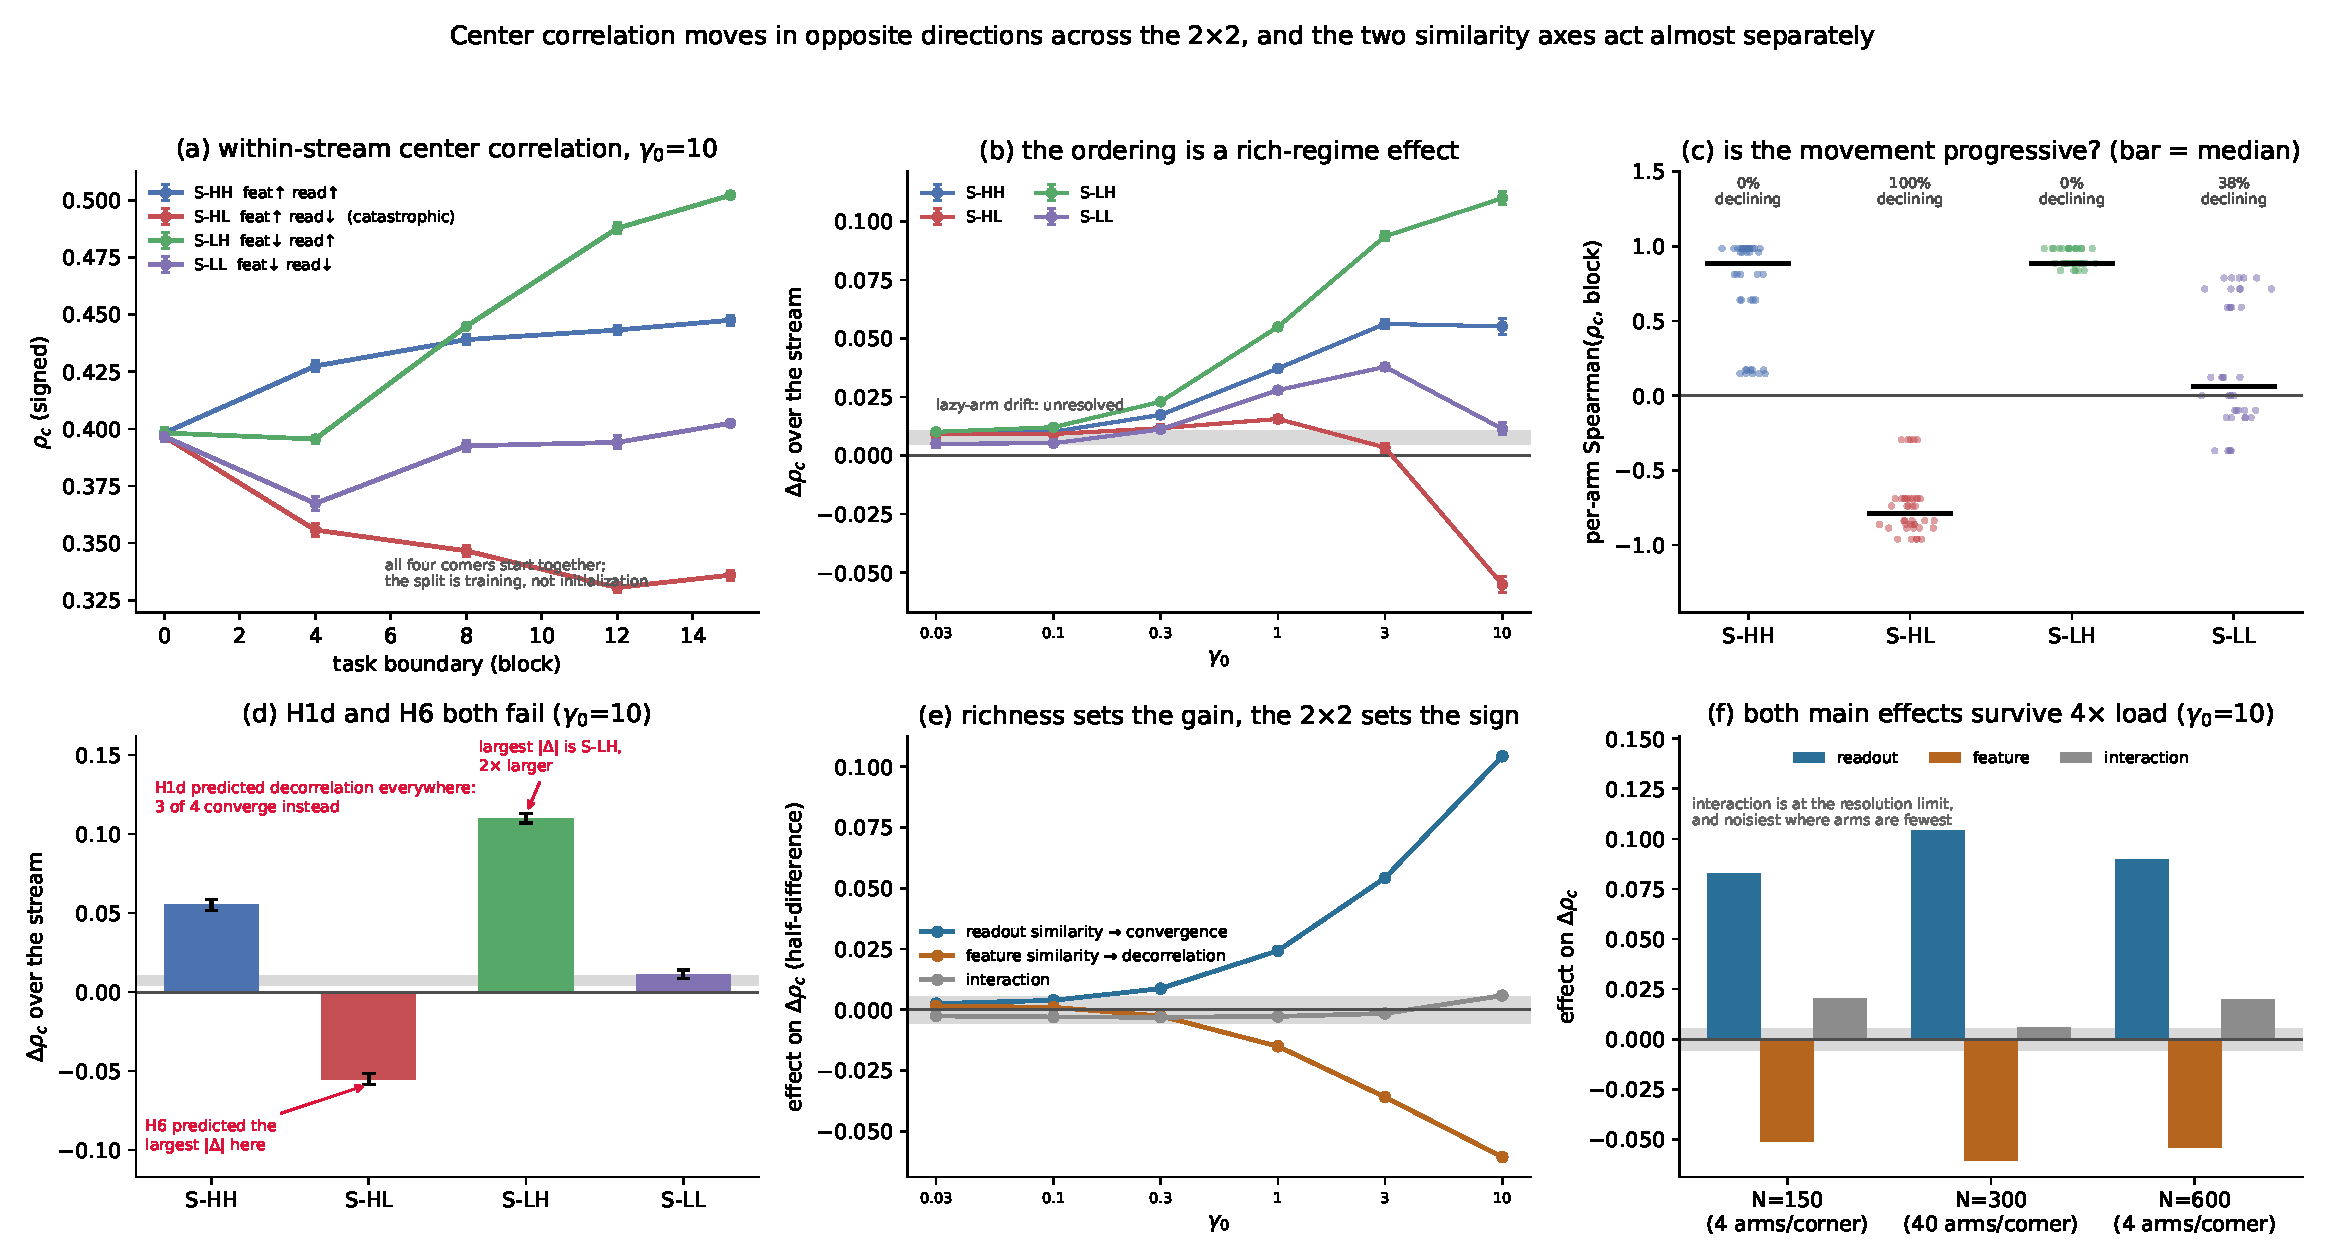
\includegraphics[width=\linewidth]
   {figures/fig4_corners_rho_c__gamma10__960arms__8dd793134c38.pdf}}
\end{figure}
